%\pdfoutput=1
%\input{style.tex}
\documentclass[letterpaper,useAMS,usenatbib]{mn2e}
\usepackage[colorlinks=true,
            linkcolor=blue,
            urlcolor=blue,
					  citecolor=blue]{hyperref}
\usepackage{amssymb}
\usepackage{graphicx}
\usepackage{amsmath}
\usepackage[amssymb]{SIunits} 
\usepackage{booktabs}
\usepackage{hhline}
\usepackage{breqn}
\usepackage{standalone}
\usepackage{dcolumn}
	\newcolumntype{d}[1]{D{.}{.}{#1}}
\usepackage{tabularx}
\usepackage{booktabs}
\usepackage{microtype}
\graphicspath{{figures/drafts/}{figures/finalized}}
\newcommand{\mc}[1]{\multicolumn{1}{c}{#1}} % handy shortcut macro
%-----------------------------------------------------------------------
\def\apjl{ApJL }
\def\aj{AJ }
\def\apj{ApJ }
\def\pasp{PASP }
\def\spie{SPIE }
\def\apjs{ApJS }
\def\araa{ARAA }
\def\aap{A\&A }
\def\nat{Nature }
\def\mnras{MNRAS }
\def\mnrasl{MNRASL }
\providecommand{\eprint}[1]{\href{http://arxiv.org/abs/#1}{#1}}
\providecommand{\adsurl}[1]{\href{#1}{ADS}}
\providecommand{\ISBN}[1]{\href{http://cosmologist.info/ISBN/#1}{ISBN: #1}} 
%-----------------------------------------------------------------------
\title[
	Galaxy-dark matter offsets in galaxy clusters and groups of the
Illustris simulation
]
{Plots: Galaxy-dark matter offsets in galaxy clusters and groups of the
Illustris simulation}
\author[Karen Y. Ng et al.]{Karen Y. Ng,$^{1}$
	Annalisa P. Pillepich,$^{2}$ 
	William A. Dawson,$^{3}$ 
	D. Wittman,$^{1}$
	\newauthor Lars Hernquist,$^{2}$
	etc. [order TBD]
}
\begin{document}
\date{arXiv} \pagerange{\pageref{firstpage}--\pageref{lastpage}}
\pubyear{2015} \maketitle\label{firstpage}
\begin{abstract} 
\end{abstract}
\begin{keywords}
	galaxy clusters, dark matter, something else 
\end{keywords}
\begin{figure*}
	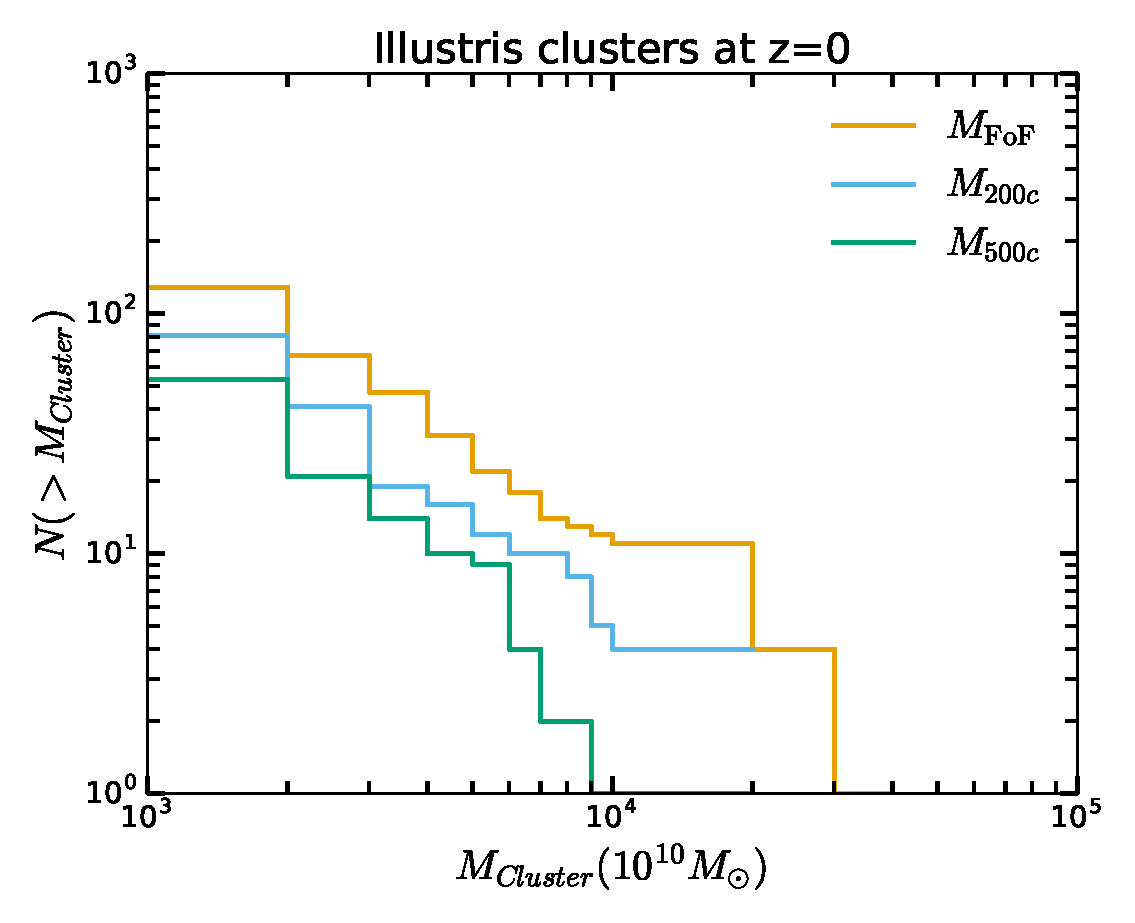
\includegraphics[width=.95\linewidth]{clusterMassDist.eps}
	\caption{
		\label{fig:config}}
\end{figure*}
\begin{figure*}
	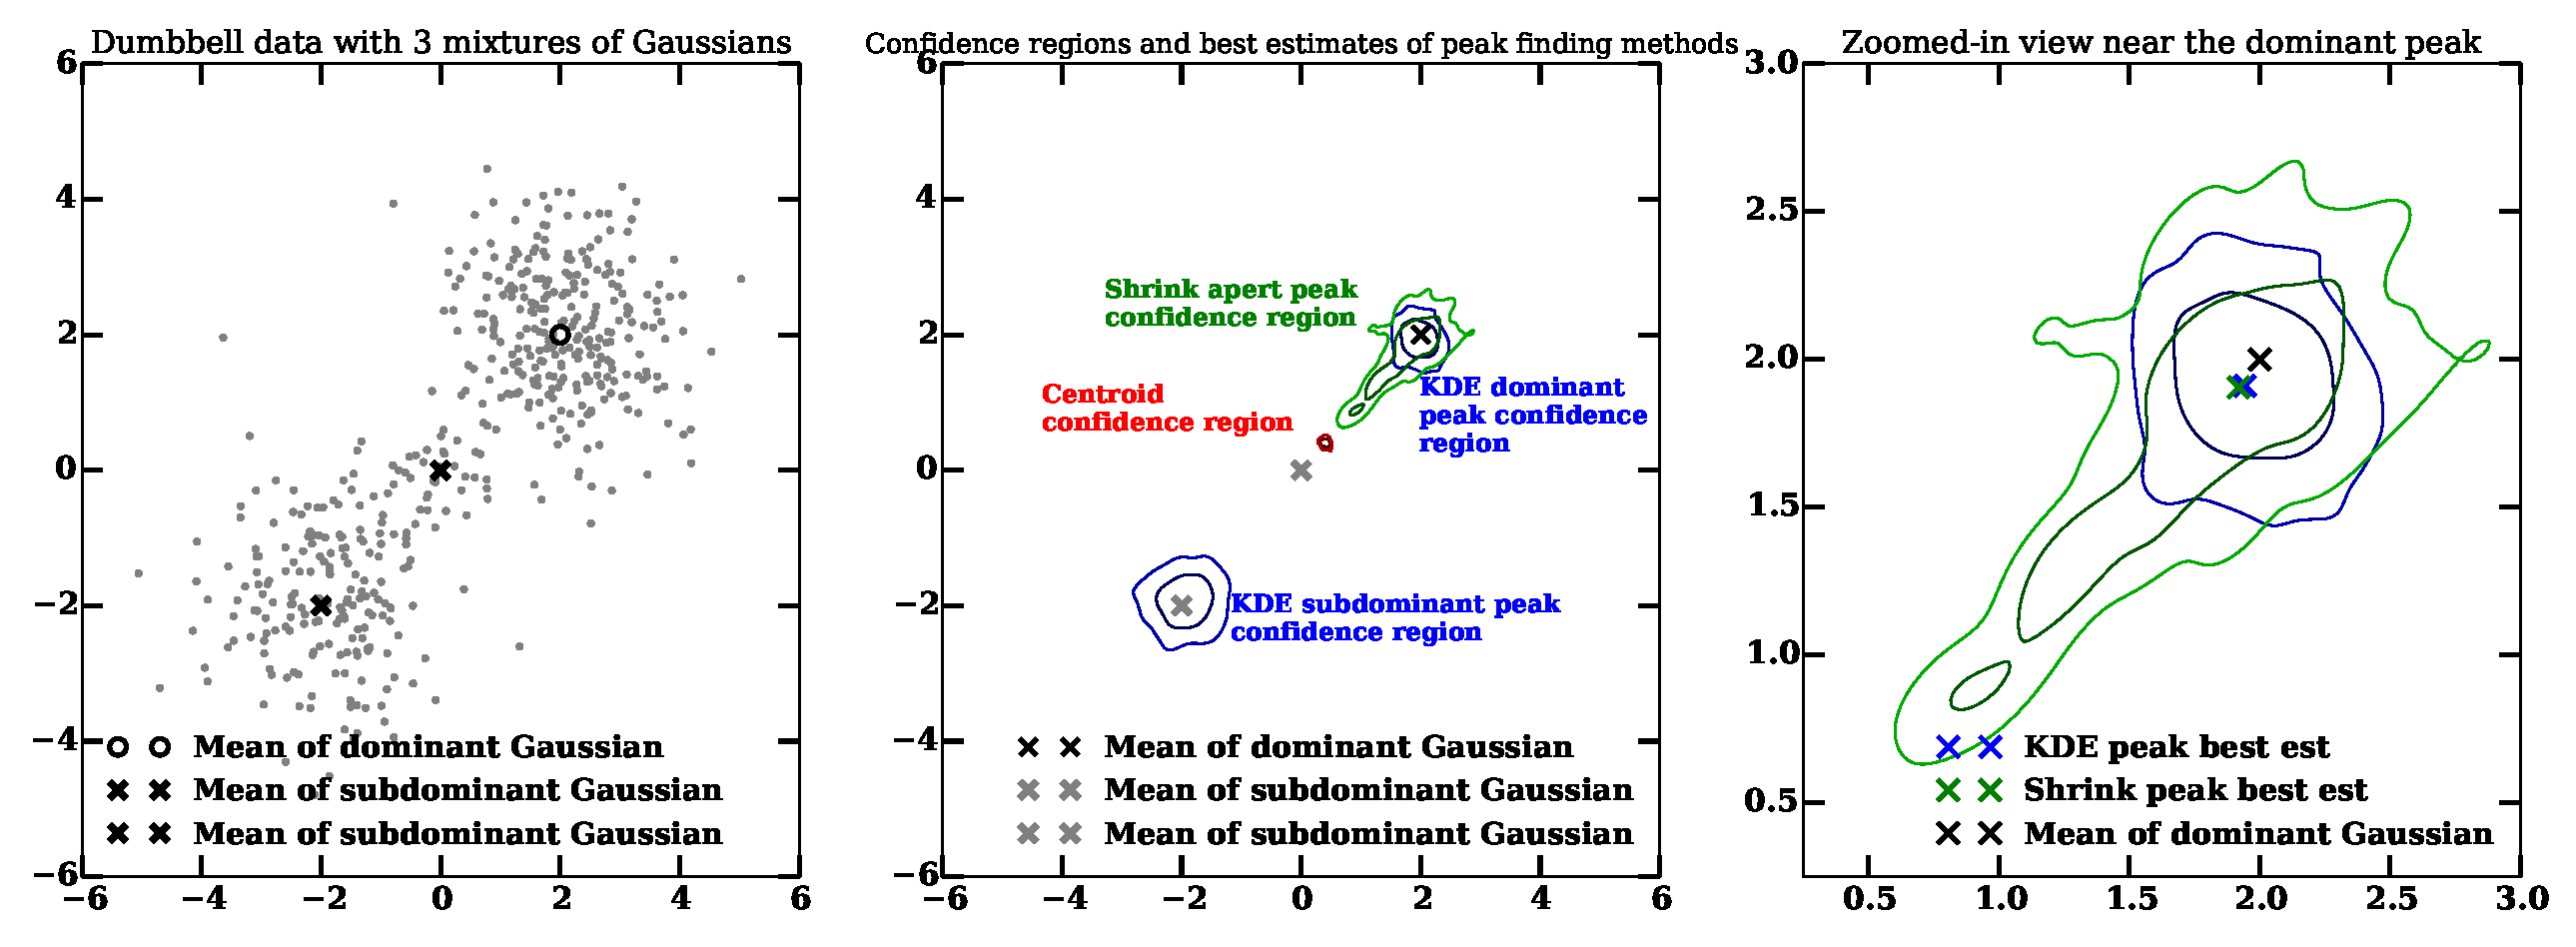
\includegraphics[width=.95\linewidth]{confidence_regions_dumbbell_500.eps}
	\caption{Comparison of the estimates given by different peak finding methods.
		{\bf Leftmost plot:} One realization of drawing data from 3 Gaussian
		mixtures. Grey data points (500 in total) were drawn from three
		Gaussian mixtures with the mean locations of the Gaussians indicated by the
		black markers. In total 200 realizations of the Gaussian data were drawn.
		{\bf Middle plot:} Each set of colored contours represents the
		68\% (inner contour) and the 95\% confidence region of the best estimates
		of the peak location. The contours are computed from 200 realizations of the Gaussian
		mixtures data respectively. {\bf Rightmost plot:} Zoomed-in view of the
		contours and best estimates (best est) from each method near the dominant peak.  
		\label{fig:dumbbell500}}
\end{figure*}
\clearpage\bsp\label{lastpage} 
\end{document}
